\documentclass[12pt,a4paper]{article}

% ── Língua e codificação ──────────────────────────────────────────────────────
\usepackage[portuguese]{babel}
\usepackage[utf8]{inputenc}
\usepackage[T1]{fontenc}

% ── Layout ────────────────────────────────────────────────────────────────────
\usepackage[top=2.5cm, bottom=2.5cm, left=3cm, right=3cm]{geometry}
\usepackage{setspace}
\usepackage{parskip}
\setlength{\parindent}{0pt}
\setlength{\parskip}{0.6em}

% ── Matemática ────────────────────────────────────────────────────────────────
\usepackage{amsmath}
\usepackage{amssymb}

% ── Gráficos ──────────────────────────────────────────────────────────────────
\usepackage{graphicx}
\usepackage{subcaption}
\usepackage{float}
\graphicspath{{./}}

% ── Tabelas ───────────────────────────────────────────────────────────────────
\usepackage{booktabs}
\usepackage{multirow}
\usepackage{array}
\usepackage{tabularx}

% ── Cores e Hiperligações ─────────────────────────────────────────────────────
\usepackage{xcolor}
\usepackage[
  colorlinks=true,
  linkcolor=blue!60!black,
  citecolor=blue!60!black,
  urlcolor=blue!60!black
]{hyperref}

% ── Captions ─────────────────────────────────────────────────────────────────
\usepackage[labelfont=bf, font=small]{caption}

% ── Macros para nomes de ficheiros com % ─────────────────────────────────────
% O catcode de % muda para "outro" (12) dentro do grupo, permitindo usá-lo
% em nomes de ficheiros. Os \gdef são globais e persistem fora do grupo.
\begingroup
\catcode`\%=12\relax
\gdef\imgLossVAE{lossGraphVAE100%.png}
\gdef\imgAnaliseMetricas{analiseMetricas100%.png}
\endgroup

% ─────────────────────────────────────────────────────────────────────────────
\begin{document}

% ══ CAPA ══════════════════════════════════════════════════════════════════════
\begin{titlepage}
  \centering
  \vspace*{1.5cm}

  {\scshape\Large Universidade — Inteligência Artificial Generativa\par}
  \vspace{0.5cm}
  \rule{\linewidth}{0.5pt}\\[0.4cm]
  {\huge\bfseries Trabalho Prático 1\\[0.3em]
  Comparação de Modelos Generativos\\no Dataset ArtBench-10\par}
  \rule{\linewidth}{0.5pt}\\[1.5cm]

  {\large
  \textbf{Autor(es):} [Nome(s) do(s) Autor(es)]\\[0.3em]
  \textbf{Número(s):} [Número(s) de Aluno]\\[0.3em]
  \textbf{Docente:} [Nome do Docente]\\[1.5cm]
  Abril 2026\par}

  \vfill
\end{titlepage}

% ══ RESUMO ════════════════════════════════════════════════════════════════════
\begin{abstract}
\noindent
Este relatório descreve o desenvolvimento e avaliação comparativa de três modelos
generativos de imagens — Autoencoder Variacional (VAE), Rede Adversarial Convolucional
Profunda (DCGAN) e Modelo de Difusão por Desruído por Pontuação (DDPM) — treinados
no dataset completo ArtBench-10 (50\,000 imagens de treino, 32$\times$32 píxeis,
10 estilos artísticos). A avaliação quantitativa baseia-se nas métricas
\textit{Fréchet Inception Distance} (FID) e \textit{Kernel Inception Distance} (KID),
calculadas para 10 sementes aleatórias com 5\,000 amostras geradas por modelo.
O DCGAN obteve o melhor desempenho (FID\,=\,$30{,}46\pm 0{,}57$;
KID\,=\,$0{,}0032\pm 0{,}0001$), seguido pelo DDPM
(FID\,=\,$37{,}91\pm 0{,}37$; KID\,=\,$0{,}0062\pm 0{,}0002$) e pelo VAE
(FID\,=\,$140{,}37\pm 0{,}43$; KID\,=\,$0{,}0314\pm 0{,}0004$). Os resultados
demonstram que, para imagens de baixa resolução (32$\times$32), um GAN bem afinado
pode superar métricas de modelos de difusão com amostragem DDIM acelerada,
embora visualmente o DDPM exiba maior diversidade de conteúdo.
\end{abstract}

\tableofcontents
\newpage

% ══ 1. INTRODUÇÃO ═════════════════════════════════════════════════════════════
\section{Introdução}

Os modelos generativos de imagens progrediram enormemente na última década, passando
de architecturas simples para sistemas capazes de sintetizar imagens foto-realistas
e artisticamente coerentes. Três paradigmas dominam actualmente a literatura:
os Autoencoders Variacionais (VAE)~\cite{kingma2013vae}, as Redes Adversariais
Generativas (GAN)~\cite{goodfellow2014gans} e, mais recentemente, os Modelos de
Difusão~\cite{ho2020ddpm}. Cada paradigma impõe compromissos distintos entre
qualidade amostral, diversidade, velocidade de treino e de inferência.

Este trabalho tem como objectivos:
\begin{enumerate}
  \item Implementar e treinar três modelos generativos no dataset \textbf{ArtBench-10}
        \cite{liao2022artbench}: um VAE convolucional (\textit{ConvVAE}), um DCGAN
        \cite{radford2015dcgan} e um DDPM baseado em U-Net com atenção
        \cite{ho2020ddpm};
  \item Avaliar quantitativamente a qualidade das amostras geradas usando FID
        \cite{heusel2017fid} e KID \cite{binkowski2018kid};
  \item Comparar e discutir os resultados obtidos.
\end{enumerate}

Todos os modelos foram treinados no dataset completo (100\%) e avaliados com um
protocolo rigoroso de 10 sementes para garantir robustez estatística.

% ══ 2. DATASET ════════════════════════════════════════════════════════════════
\section{Dataset: ArtBench-10}

O \textbf{ArtBench-10}~\cite{liao2022artbench} é um dataset público de obras de arte
agrupadas em 10 estilos históricos:
\textit{Art Nouveau}, \textit{Baroque}, \textit{Expressionism},
\textit{Impressionism}, \textit{Post-Impressionism}, \textit{Realism},
\textit{Renaissance}, \textit{Romanticism}, \textit{Surrealism} e
\textit{Ukiyo-e}.
O dataset está balanceado, com 5\,000 imagens de treino e 1\,000 de teste por classe,
totalizando \textbf{50\,000 imagens de treino} e \textbf{10\,000 de teste}.

Para este trabalho, todas as imagens foram redimensionadas para $32\times32$ píxeis
e normalizadas. Dependendo do modelo, a normalização foi feita para $[0, 1]$
(VAE, que usa função de activação Sigmoid no decoder) ou para $[-1, 1]$
(DCGAN e DDPM, que usam Tanh e normalização padrão, respectivamente).
O DDPM aplicou adicionalmente \textit{data augmentation}: \textit{RandomCrop}
com margem de 4 píxeis, \textit{RandomHorizontalFlip} ($p=0{,}5$) e
\textit{ColorJitter} ligeiro (brilho/contraste/saturação $\pm5\%$, tonalidade $\pm2\%$).

% ══ 3. MODELOS GENERATIVOS ════════════════════════════════════════════════════
\section{Modelos Generativos}

\subsection{Autoencoder Variacional (VAE)}

\subsubsection*{Fundamento Teórico}

O VAE~\cite{kingma2013vae} aprende a distribuição latente dos dados maximizando
a \textit{Evidence Lower BOund} (ELBO):
\begin{equation}
  \mathcal{L}(\theta, \phi;\, x) =
    \underbrace{\mathbb{E}_{q_\phi(z|x)}\bigl[\log p_\theta(x|z)\bigr]}_{\text{reconstrução}}
    - \underbrace{D_{\mathrm{KL}}\bigl(q_\phi(z|x)\,\|\,p(z)\bigr)}_{\text{regularização}},
\end{equation}
onde $q_\phi(z|x) = \mathcal{N}\bigl(\mu_\phi(x),\,\sigma^2_\phi(x)\,I\bigr)$
é o encoder e $p(z) = \mathcal{N}(0, I)$ o prior.
O \textit{reparameterization trick} ($z = \mu + \sigma \odot \varepsilon$,
$\varepsilon \sim \mathcal{N}(0,I)$) permite diferenciar através da amostragem.

O modelo usa a variante $\beta$-VAE~\cite{higgins2017betavae} com $\beta < 1$
para dar mais peso à reconstrução:
\begin{equation}
  \mathcal{L}_\beta = \mathcal{L}_{\mathrm{recon}} - \beta\,D_{\mathrm{KL}},
  \quad \beta = 0{,}5.
\end{equation}

\subsubsection*{Arquitectura}

O \textbf{encoder} é composto por três blocos convolucionais com \textit{stride} 2
(canais: $3 \to 64 \to 128 \to 256$), seguidos de \textit{BatchNorm} e
\textit{LeakyReLU}$(0{,}2)$. A representação é projectada para $\mu$ e
$\log \sigma^2$ por duas camadas lineares ($256 \cdot 4 \cdot 4 \to 128$).

O \textbf{decoder} inverte o processo: uma camada linear ($128 \to 256 \cdot 4 \cdot 4$)
alimenta três \textit{ConvTranspose2d} (canais: $256 \to 128 \to 64 \to 3$)
com \textit{BatchNorm}, \textit{ReLU} e \textit{Sigmoid} na saída.

\subsubsection*{Treino}

\begin{itemize}
  \item \textbf{Épocas:} 100 \quad \textbf{Batch:} 64 \quad \textbf{Optimizador:} Adam ($\eta=10^{-3}$)
  \item \textbf{Perda de reconstrução:} BCE (soma normalizada pelo batch)
  \item \textbf{Perda KL:} $-0{,}5\sum(1 + \log\sigma^2 - \mu^2 - \sigma^2)$
\end{itemize}

A curva de treino (Figura~\ref{fig:vae_loss}) mostra convergência estável:
a perda total desceu de $\approx 1840$ para $\approx 1780$, com a reconstrução
a dominar ($\approx 1755$ no final) e a divergência KL a estabilizar em $\approx 65$,
indicando que o modelo aprendeu uma representação latente informativa.

\begin{figure}[H]
  \centering
  \includegraphics[width=0.92\linewidth]{\imgLossVAE}
  \caption{Curvas de treino do VAE: perda total, perda de reconstrução (BCE) e
           divergência KL ao longo de 100 épocas.}
  \label{fig:vae_loss}
\end{figure}

\subsection{Rede Adversarial Convolucional Profunda (DCGAN)}

\subsubsection*{Fundamento Teórico}

As GAN~\cite{goodfellow2014gans} formulam o treino como um jogo minimax entre
um gerador $G$ e um discriminador $D$:
\begin{equation}
  \min_G \max_D\; \mathbb{E}_{x \sim p_{\mathrm{data}}}[\log D(x)]
  + \mathbb{E}_{z \sim p_z}[\log(1 - D(G(z)))].
\end{equation}
Na prática, o gerador maximiza $\mathbb{E}_z[\log D(G(z))]$ para evitar gradientes
saturados durante o treino inicial.

O DCGAN~\cite{radford2015dcgan} impõe restrições arquitectónicas que estabilizam
o treino: convoluções com \textit{stride} no discriminador (em vez de
\textit{max-pooling}), \textit{ConvTranspose2d} no gerador,
\textit{BatchNorm} em todas as camadas e \textit{LeakyReLU} no discriminador.

\subsubsection*{Arquitectura}

O \textbf{gerador} transforma um vector de ruído
$z \in \mathbb{R}^{100}$ em imagem $3 \times 32 \times 32$:
\begin{equation*}
  z \;(100 \times 1 \times 1)
  \xrightarrow{512 \times 4 \times 4}
  \xrightarrow{256 \times 8 \times 8}
  \xrightarrow{128 \times 16 \times 16}
  \xrightarrow{3 \times 32 \times 32 \;\text{Tanh}}
\end{equation*}
com \textit{BatchNorm} + \textit{ReLU} em cada bloco intermédio.

O \textbf{discriminador} inverte este percurso:
\begin{equation*}
  3 \times 32 \times 32
  \xrightarrow{64}
  \xrightarrow{128}
  \xrightarrow{256}
  \xrightarrow{1 \;\text{Sigmoid}}
\end{equation*}
com \textit{LeakyReLU}$(0{,}2)$ em cada bloco.

\subsubsection*{Treino}

\begin{itemize}
  \item \textbf{Épocas:} 200 \quad \textbf{Batch:} 64
  \item \textbf{Optimizador (G e D):} Adam ($\eta = 2 \times 10^{-4}$, $\beta_1 = 0{,}5$)
  \item \textbf{\textit{Label smoothing}:} rótulos reais $= 0{,}9$ (estabiliza o discriminador)
  \item \textbf{Inicialização:} $\mathcal{N}(0, 0{,}02)$ para pesos convolucionais,
        $\mathcal{N}(1, 0{,}02)$ para $\gamma$ do \textit{BatchNorm}
\end{itemize}

\subsection{Modelo de Difusão por Desruído (DDPM)}

\subsubsection*{Fundamento Teórico}

Os DDPM~\cite{ho2020ddpm} definem um processo de difusão directo (adição progressiva
de ruído) e aprendem o processo inverso (remoção de ruído). O processo directo é:
\begin{equation}
  q(x_t | x_{t-1}) = \mathcal{N}\!\left(x_t;\,\sqrt{1-\beta_t}\,x_{t-1},\,\beta_t I\right),
\end{equation}
o que permite amostrar directamente:
\begin{equation}
  q(x_t | x_0) = \mathcal{N}\!\left(x_t;\,\sqrt{\bar\alpha_t}\,x_0,\,(1-\bar\alpha_t)I\right),
  \quad \bar\alpha_t = \prod_{s=1}^{t}(1-\beta_s).
\end{equation}
O modelo $\epsilon_\theta$ é treinado para prever o ruído adicionado:
\begin{equation}
  \mathcal{L} = \mathbb{E}_{t,\,x_0,\,\epsilon}\!\left[
    \bigl\|\epsilon - \epsilon_\theta\!\left(\sqrt{\bar\alpha_t}\,x_0
    + \sqrt{1-\bar\alpha_t}\,\epsilon,\;t\right)\bigr\|^2\right].
\end{equation}
Para inferência eficiente, foi usado o esquema \textbf{DDIM}~\cite{song2020ddim}
com 100 passos (em vez dos 1000 do treino), reduzindo o tempo de geração de
$\sim$90 min para $\sim$10 min por 5\,000 amostras.

\subsubsection*{Arquitectura: U-Net com Auto-atenção}

A U-Net (\textbf{29,60 M parâmetros}, $\texttt{BASE\_CH}=128$, $\texttt{T\_DIM}=256$)
opera em três níveis de resolução ($32 \to 16 \to 8$ píxeis):

\begin{itemize}
  \item \textbf{Encoder:} dois \textit{ResBlocks} por nível; \textit{SelfAttention}
        de 4 cabeças nas resoluções $16\times16$ e $8\times8$.
  \item \textbf{Bottleneck ($8\times8$):} \textit{ResBlock} + \textit{SelfAttention}
        + \textit{ResBlock}.
  \item \textbf{Decoder:} \textit{Upsample} + concatenação com \textit{skip connection}
        + dois \textit{ResBlocks} (+ \textit{SelfAttention} a $16\times16$).
  \item \textbf{ResBlock:} \textit{GroupNorm} + \textit{SiLU} + \textit{Conv2d}
        $3\times3$, projecção da incorporação temporal $t$ por camada linear,
        \textit{Dropout}$(0{,}1)$ e ligação residual.
  \item \textbf{Incorporação temporal:} \textit{Sinusoidal Positional Encoding}
        seguido de MLP de duas camadas ($t\_\mathrm{dim} \to 2\,t\_\mathrm{dim}
        \to t\_\mathrm{dim}$).
  \item \textbf{Inicialização zero} na última convolução (estabiliza o início do treino).
\end{itemize}

\subsubsection*{Treino}

\begin{itemize}
  \item \textbf{Épocas:} 500 \quad \textbf{Batch:} 128 \quad \textbf{Steps totais:} 195\,000
  \item \textbf{Optimizador:} AdamW ($\eta = 2 \times 10^{-4}$, sem \textit{weight decay})
  \item \textbf{LR schedule:} \textit{warmup} linear (10 épocas) + decaimento cosseno
        suave ($\eta_{\min} = 0{,}1\,\eta_0$)
  \item \textbf{Clipping de gradiente:} norma máxima de $1{,}0$
  \item \textbf{EMA} (\textit{Exponential Moving Average}) dos pesos com
        $\text{decay} = 0{,}9995$ (usado exclusivamente na amostragem)
  \item \textbf{Escalonamento linear de $\beta$:}
        $\beta_1 = 10^{-4}$, $\beta_T = 0{,}02$, $T = 1000$;
        $\bar\alpha_T \approx 4 \times 10^{-5}$ (ruído quase puro)
\end{itemize}

% ══ 4. PROTOCOLO DE AVALIAÇÃO ═════════════════════════════════════════════════
\section{Protocolo de Avaliação}

\subsection*{Métricas}

\paragraph{FID — \textit{Fréchet Inception Distance}~\cite{heusel2017fid}.}
Mede a distância entre as distribuições real e gerada no espaço de
características do InceptionV3:
\begin{equation}
  \mathrm{FID} = \|\mu_r - \mu_g\|^2
    + \mathrm{Tr}\!\left(\Sigma_r + \Sigma_g - 2\,(\Sigma_r\Sigma_g)^{1/2}\right).
\end{equation}
Valores mais baixos indicam maior semelhança estatística com os dados reais.

\paragraph{KID — \textit{Kernel Inception Distance}~\cite{binkowski2018kid}.}
Estima a \textit{Maximum Mean Discrepancy} (MMD) com \textit{kernel} RBF
entre as distribuições de características do InceptionV3:
\begin{equation}
  \mathrm{KID} = \mathrm{MMD}^2(P_r, P_g).
\end{equation}
É calculado por média de 50 \textit{subsets} de tamanho 100 e, ao contrário do
FID, tem um estimador não enviesado, sendo mais robusto para amostras pequenas.

\subsection*{Protocolo}

\begin{enumerate}
  \item \textbf{Amostras:} 5\,000 imagens geradas e 5\,000 reais (test set),
        por cada uma das 10 sementes (42–51).
  \item \textbf{Pré-processamento:} imagens redimensionadas para $299\times299$
        e normalizadas para $[-1, 1]$ antes da extracção de características.
  \item \textbf{InceptionV3} pré-treinado no ImageNet (fc substituída por
        \texttt{Identity}) fornece vectores de $2048$ dimensões.
  \item \textbf{FID} calculado sobre as 5\,000 características completas;
        \textbf{KID} calculado sobre 50 \textit{subsets} de 100 amostras.
  \item \textbf{Amostragem DDIM} (100 passos) para o DDPM — mesmos pesos,
        estratégia de inferência mais rápida.
\end{enumerate}

% ══ 5. RESULTADOS ═════════════════════════════════════════════════════════════
\section{Resultados}

\subsection{Análise Qualitativa}

A Figura~\ref{fig:amostras} apresenta grelhas de 64 amostras geradas por cada
modelo após treino no dataset completo.

\begin{figure}[H]
  \centering
  \begin{subfigure}[t]{0.32\linewidth}
    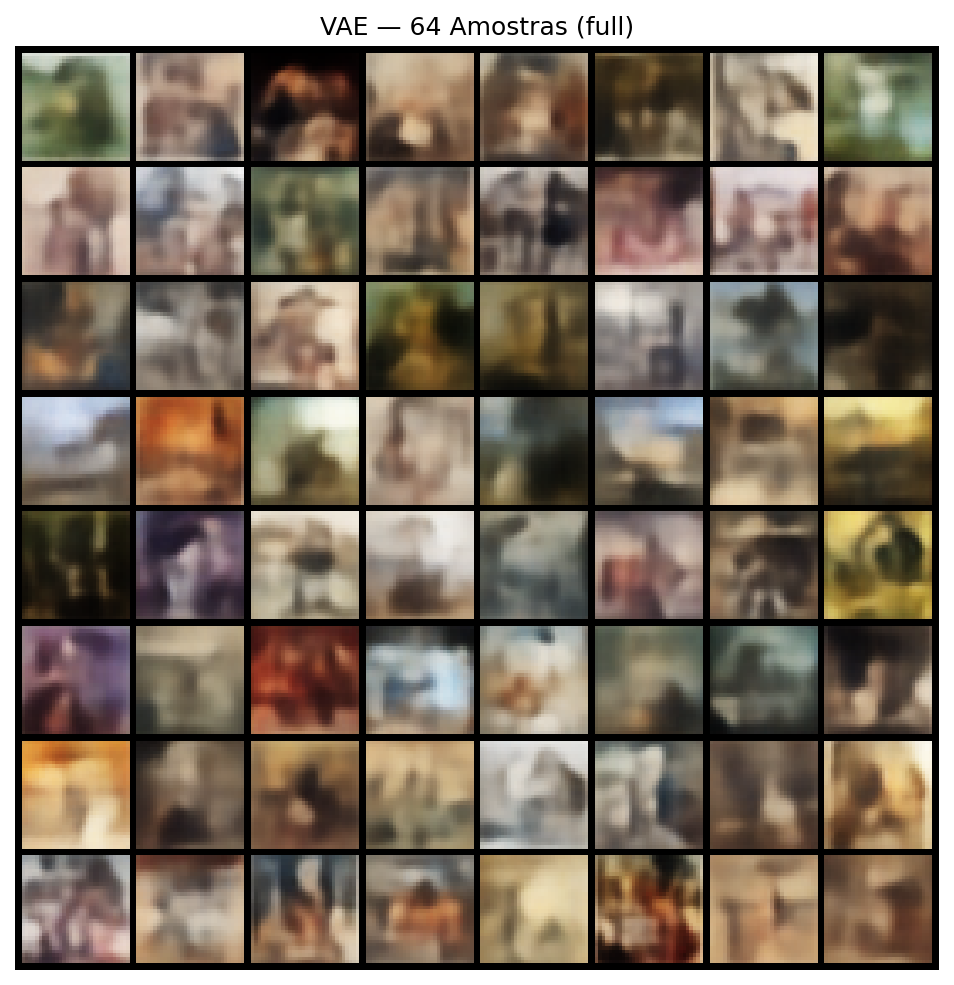
\includegraphics[width=\linewidth]{amostras_vae_full.png}
    \caption{VAE}
  \end{subfigure}
  \hfill
  \begin{subfigure}[t]{0.32\linewidth}
    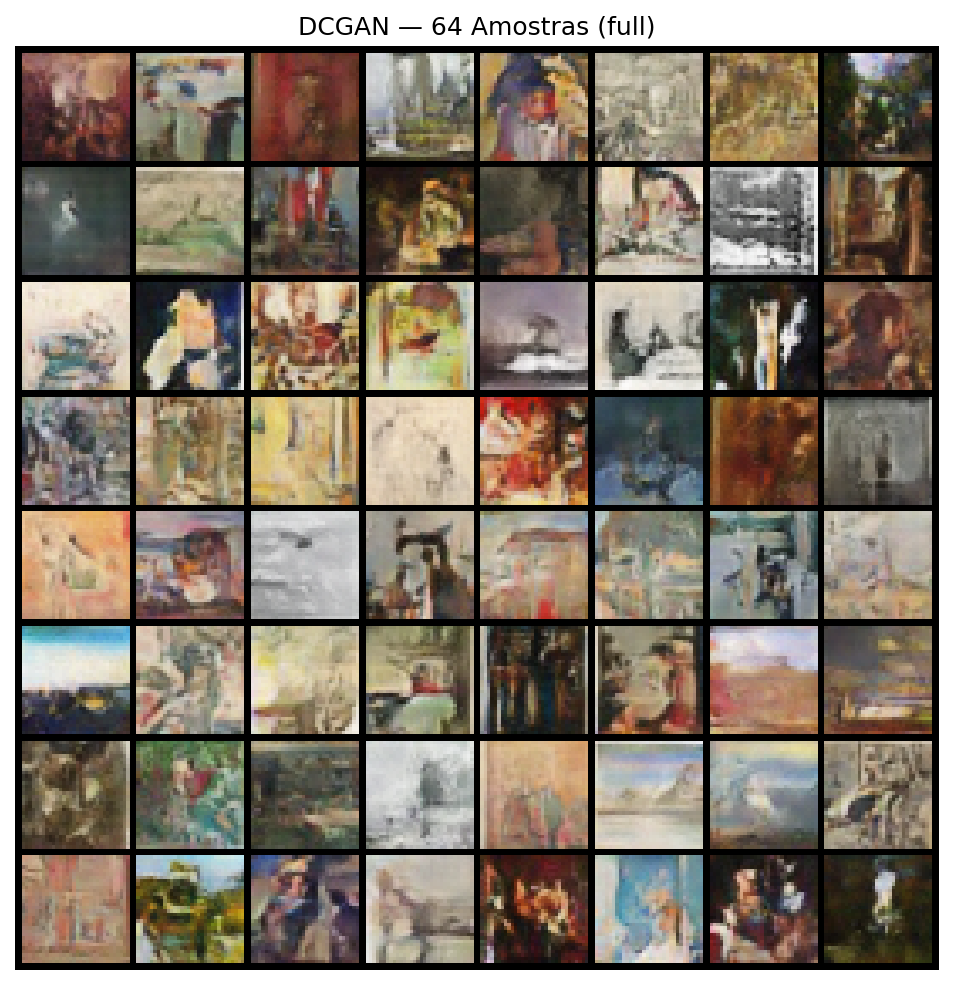
\includegraphics[width=\linewidth]{amostras_gan_full.png}
    \caption{DCGAN}
  \end{subfigure}
  \hfill
  \begin{subfigure}[t]{0.32\linewidth}
    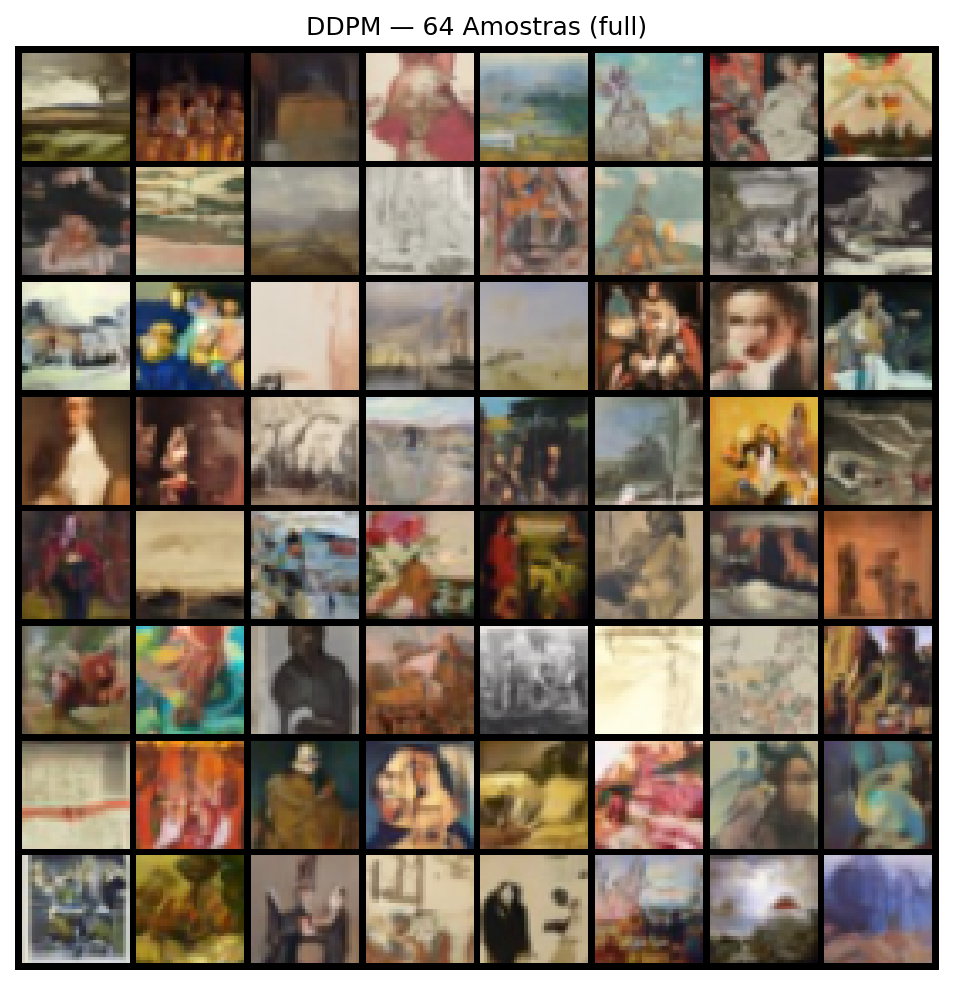
\includegraphics[width=\linewidth]{amostras_diffusion_full.png}
    \caption{DDPM}
  \end{subfigure}
  \caption{64 amostras geradas por cada modelo (dataset completo, 32$\times$32 píxeis).
           O VAE produz imagens com aspecto desfocado característico da suavização
           imposta pela perda de reconstrução. O DCGAN gera imagens mais nítidas mas
           com alguma repetição de padrões. O DDPM exibe a maior variabilidade de
           conteúdo e estilo artístico.}
  \label{fig:amostras}
\end{figure}

\subsection{Análise Quantitativa}

\subsubsection*{Resultados Globais}

A Tabela~\ref{tab:resultados} resume os resultados finais, calculados como
média $\pm$ desvio padrão sobre 10 sementes.

\begin{table}[H]
  \centering
  \caption{FID e KID (média $\pm$ desvio padrão, 10 sementes) para os três modelos
           treinados no dataset completo. Valores mais baixos indicam melhor qualidade.}
  \label{tab:resultados}
  \begin{tabular}{lccc}
    \toprule
    \textbf{Modelo} & \textbf{FID} ($\downarrow$) & \textbf{KID} ($\downarrow$) \\
    \midrule
    VAE   & $140{,}37 \pm 0{,}43$ & $0{,}0314 \pm 0{,}0004$ \\
    DCGAN & $\mathbf{30{,}46 \pm 0{,}57}$ & $\mathbf{0{,}0032 \pm 0{,}0001}$ \\
    DDPM  & $37{,}91 \pm 0{,}37$ & $0{,}0062 \pm 0{,}0002$ \\
    \bottomrule
  \end{tabular}
\end{table}

A Figura~\ref{fig:metricas} ilustra visualmente a separação entre os três modelos.

\begin{figure}[H]
  \centering
  \includegraphics[width=0.95\linewidth]{\imgAnaliseMetricas}
  \caption{Comparação de FID e KID para os três modelos (barras de erro = desvio padrão
           sobre 10 sementes). O DCGAN supera os restantes modelos em ambas as métricas.}
  \label{fig:metricas}
\end{figure}

\subsubsection*{Resultados por Semente}

A Tabela~\ref{tab:sementes} detalha os resultados por semente, permitindo avaliar
a estabilidade das métricas.

\begin{table}[H]
  \centering
  \caption{FID e KID por semente para os três modelos (dataset completo).}
  \label{tab:sementes}
  \setlength{\tabcolsep}{5pt}
  \begin{tabular}{c rr r rr r}
    \toprule
    & \multicolumn{3}{c}{\textbf{FID}} & \multicolumn{3}{c}{\textbf{KID}} \\
    \cmidrule(lr){2-4}\cmidrule(lr){5-7}
    \textbf{Semente} & VAE & DCGAN & DDPM & VAE & DCGAN & DDPM \\
    \midrule
    42 & 140,66 & 31,10 & 37,91 & 0,0315 & 0,0032 & 0,0061 \\
    43 & 140,34 & 29,56 & 38,35 & 0,0315 & 0,0033 & 0,0065 \\
    44 & 139,59 & 29,91 & 37,63 & 0,0311 & 0,0031 & 0,0063 \\
    45 & 140,29 & 30,29 & 37,88 & 0,0315 & 0,0032 & 0,0063 \\
    46 & 140,34 & 30,23 & 38,05 & 0,0306 & 0,0032 & 0,0063 \\
    47 & 141,28 & 31,35 & 37,39 & 0,0321 & 0,0033 & 0,0059 \\
    48 & 140,76 & 30,87 & 38,29 & 0,0315 & 0,0034 & 0,0063 \\
    49 & 140,07 & 30,70 & 37,20 & 0,0314 & 0,0032 & 0,0060 \\
    50 & 140,26 & 29,73 & 38,04 & 0,0319 & 0,0030 & 0,0062 \\
    51 & 140,08 & 30,82 & 38,33 & 0,0311 & 0,0032 & 0,0062 \\
    \midrule
    \textbf{Média} & \textbf{140,37} & \textbf{30,46} & \textbf{37,91}
                   & \textbf{0,0314} & \textbf{0,0032} & \textbf{0,0062} \\
    \textbf{Std}   & 0,43 & 0,57 & 0,37 & 0,0004 & 0,0001 & 0,0002 \\
    \bottomrule
  \end{tabular}
\end{table}

% ══ 6. DISCUSSÃO ══════════════════════════════════════════════════════════════
\section{Discussão}

\paragraph{VAE — Limitações da perda de reconstrução.}
O VAE obteve os piores resultados em ambas as métricas (FID $\approx$ 140,37).
A causa principal é a suavização intrínseca da perda BCE pixel-a-pixel: ao
minimizar o erro médio de reconstrução, o modelo aprende a gerar imagens com
aparência desfocada (\textit{blurry}), já que a média de distribuições nítidas
mas díspares é uma imagem desfocada. O espaço latente contínuo e regular facilita
interpolação, mas não garante qualidade perceptual. Adicionalmente, a resolução
reduzida (32$\times$32) amplifica este efeito, pois os detalhes de alta frequência
perdem-se facilmente na compressão para $z \in \mathbb{R}^{128}$.

\paragraph{DCGAN — Melhor FID e KID.}
O DCGAN obteve o melhor desempenho em ambas as métricas. Isto deve-se ao objectivo
adversarial, que força o gerador a produzir imagens que o discriminador não consegue
distinguir das reais — ou seja, a distribuição geradora aproxima-se directamente
da distribuição real em termos perceptuais. A resolução $32\times32$ favorece os
GANs, pois a complexidade do discriminador é suficiente para cobrir o espaço de
características relevante. O \textit{label smoothing} e a inicialização cuidadosa
dos pesos contribuíram para a estabilidade do treino ao longo de 200 épocas.

No entanto, os GANs são propensos a \textit{mode dropping} — uma limitação não
visível no FID/KID mas observável nas amostras: algumas imagens da grelha do DCGAN
mostram repetição de padrões similares, sugerindo que o modelo não cobre todos os
10 estilos artísticos com igual probabilidade.

\paragraph{DDPM — Qualidade vs.\ diversidade.}
O DDPM (FID $\approx$ 37,91) ficou ligeiramente abaixo do DCGAN mas significativamente
acima do VAE. Visualmente, as amostras do DDPM exibem a maior diversidade de
conteúdo — diferentes estilos, composições e paletas de cor — o que é esperado
dada a formulação probabilística mais rica dos modelos de difusão. O FID
ligeiramente pior face ao DCGAN pode ser atribuído a dois factores:

\begin{enumerate}
  \item \textbf{DDIM com 100 passos}: a amostragem acelerada (DDIM~\cite{song2020ddim})
        introduz um compromisso entre velocidade e qualidade — 100 passos em vez
        de 1000 podem não capturar completamente a distribuição aprendida.
  \item \textbf{Menor fidelidade pontual a 32$\times$32}: ao contrário dos GANs,
        que optimizam directamente a discriminabilidade ao nível do píxel para
        esta resolução, o DDPM opera no espaço do ruído e pode distribuir
        erros de reconstrução de forma menos concentrada.
\end{enumerate}

\paragraph{Estabilidade dos resultados.}
O desvio padrão do FID é muito baixo em todos os modelos
(VAE: $\pm 0{,}43$; DCGAN: $\pm 0{,}57$; DDPM: $\pm 0{,}37$),
confirmando que 5\,000 amostras e 10 sementes são suficientes para obter estimativas
robustas. O DCGAN apresenta ligeiramente maior variância, o que é consistente
com a natureza estocástica do processo adversarial — pequenosvariações na amostra
de ruído $z$ produzem maior dispersão nas características InceptionV3.

% ══ 7. CONCLUSÃO ══════════════════════════════════════════════════════════════
\section{Conclusão}

Este trabalho comparou três paradigmas de geração de imagens no dataset ArtBench-10
ao nível de resolução $32\times32$. Os resultados quantitativos (FID e KID)
favoreceram o \textbf{DCGAN}, que combina alta fidelidade visual com treino eficiente.
O \textbf{DDPM} posiciona-se como alternativa com maior diversidade amostral, a
custo de um FID ligeiramente superior neste cenário de baixa resolução com
amostragem DDIM. O \textbf{VAE} demonstrou as limitações da geração baseada em
reconstrução pixel-a-pixel, nomeadamente a produção de imagens desfocadas.

Como trabalho futuro, seria interessante: (i) testar o DDPM com o \textit{schedule}
completo de 1000 passos para verificar se o gap face ao DCGAN se mantém;
(ii) avaliar modelos condicionais ao estilo artístico; (iii) experimentar
resoluções maiores (64$\times$64 ou 128$\times$128), onde os modelos de difusão
tipicamente superam os GANs.

% ══ REFERÊNCIAS ═══════════════════════════════════════════════════════════════
\newpage
\begin{thebibliography}{99}

\bibitem{kingma2013vae}
D.~P. Kingma e M.~Welling,
``Auto-Encoding Variational Bayes,''
\textit{2nd International Conference on Learning Representations (ICLR)}, 2014.

\bibitem{goodfellow2014gans}
I.~Goodfellow \textit{et al.},
``Generative Adversarial Nets,''
\textit{Advances in Neural Information Processing Systems (NeurIPS)}, 2014.

\bibitem{radford2015dcgan}
A.~Radford, L.~Metz e S.~Chintala,
``Unsupervised Representation Learning with Deep Convolutional Generative
Adversarial Networks,''
\textit{3rd International Conference on Learning Representations (ICLR)}, 2016.

\bibitem{ho2020ddpm}
J.~Ho, A.~Jain e P.~Abbeel,
``Denoising Diffusion Probabilistic Models,''
\textit{Advances in Neural Information Processing Systems (NeurIPS)}, 2020.

\bibitem{song2020ddim}
J.~Song, C.~Meng e S.~Ermon,
``Denoising Diffusion Implicit Models,''
\textit{9th International Conference on Learning Representations (ICLR)}, 2021.

\bibitem{heusel2017fid}
M.~Heusel \textit{et al.},
``GANs Trained by a Two Time-Scale Update Rule Converge to a Local Nash
Equilibrium,''
\textit{Advances in Neural Information Processing Systems (NeurIPS)}, 2017.

\bibitem{binkowski2018kid}
M.~Bińkowski \textit{et al.},
``Demystifying MMD GANs,''
\textit{6th International Conference on Learning Representations (ICLR)}, 2018.

\bibitem{higgins2017betavae}
I.~Higgins \textit{et al.},
``$\beta$-VAE: Learning Basic Visual Concepts with a Constrained Variational
Framework,''
\textit{5th International Conference on Learning Representations (ICLR)}, 2017.

\bibitem{liao2022artbench}
P.~Liao \textit{et al.},
``The ArtBench Dataset: Benchmarking Generalisation in Image Generation,''
\textit{arXiv:2206.11404}, 2022.

\end{thebibliography}

\end{document}
